\chapter{Virtual Memory}

\section{Introduction}

Virtual Memory is one of the most important abstractions provided by modern operating systems. It allows processes to execute as if they have access to a large, contiguous memory space, regardless of the actual amount of installed physical memory.

Virtual memory provides:

\begin{itemize}
\item Process isolation
\item Efficient memory utilization
\item Larger logical address spaces
\item Simplified programming model
\item Multiprogramming support
\end{itemize}

\section{Motivation for Virtual Memory}

Without virtual memory:

\begin{itemize}
\item Entire program must fit in RAM
\item Large applications cannot execute
\item Multiprogramming becomes difficult
\item Memory utilization decreases
\end{itemize}

With virtual memory:

\begin{itemize}
\item Only actively used portions remain in RAM
\item Large applications can run on smaller systems
\item More processes can coexist
\item Better system throughput
\end{itemize}

\begin{figure}[H]
\centering
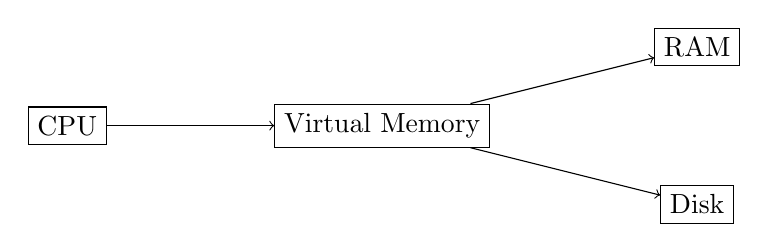
\begin{tikzpicture}
\node[draw] (cpu) at (0,0) {CPU};
\node[draw] (vm) at (4,0) {Virtual Memory};
\node[draw] (ram) at (8,1) {RAM};
\node[draw] (disk) at (8,-1) {Disk};

\draw[->] (cpu)--(vm);
\draw[->] (vm)--(ram);
\draw[->] (vm)--(disk);
\end{tikzpicture}
\caption{Virtual Memory Abstraction}
\end{figure}

\section{Virtual Address Space}

Each process sees its own virtual address space.

Typical layout:

\begin{figure}[H]
\centering
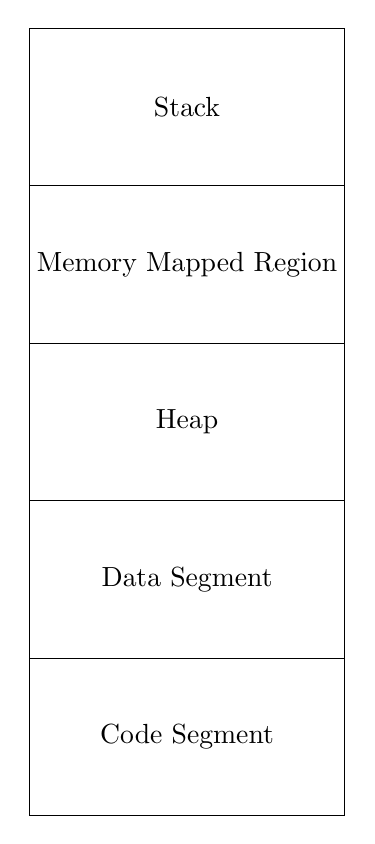
\begin{tikzpicture}
\draw (0,0) rectangle (4,10);

\draw (0,8)--(4,8);
\draw (0,6)--(4,6);
\draw (0,4)--(4,4);
\draw (0,2)--(4,2);

\node at (2,9) {Stack};
\node at (2,7) {Memory Mapped Region};
\node at (2,5) {Heap};
\node at (2,3) {Data Segment};
\node at (2,1) {Code Segment};
\end{tikzpicture}
\caption{Typical Virtual Address Space}
\end{figure}

\subsection{Advantages}

\begin{itemize}
\item Process isolation
\item Protection
\item Easier relocation
\item Shared memory support
\end{itemize}

\section{Demand Paging}

Demand paging loads pages only when required.

Instead of loading an entire program:

\begin{itemize}
\item Load minimal pages
\item Fetch remaining pages on demand
\end{itemize}

Benefits:

\begin{itemize}
\item Faster startup
\item Lower memory consumption
\item Better scalability
\end{itemize}

\begin{figure}[H]
\centering
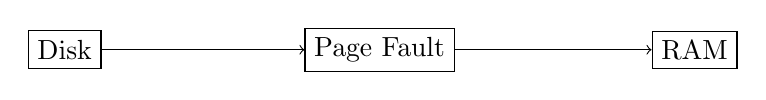
\begin{tikzpicture}
\node[draw] (disk) at (0,0) {Disk};
\node[draw] (pf) at (4,0) {Page Fault};
\node[draw] (ram) at (8,0) {RAM};

\draw[->] (disk)--(pf);
\draw[->] (pf)--(ram);
\end{tikzpicture}
\caption{Demand Paging}
\end{figure}

\section{Demand Segmentation}

Demand segmentation applies the same idea to segments.

Only required segments are loaded.

Examples:

\begin{itemize}
\item Code segment
\item Data segment
\item Shared libraries
\end{itemize}

Modern systems primarily use demand paging.

\section{Lazy Loading}

Lazy loading postpones loading until actual use.

Examples:

\begin{itemize}
\item Shared libraries
\item Dynamic modules
\item Memory mapped files
\end{itemize}

Advantages:

\begin{itemize}
\item Reduced startup time
\item Reduced memory usage
\end{itemize}

\section{Page Faults}

A page fault occurs when a process references a page that is not currently in physical memory.

\subsection{Causes}

\begin{itemize}
\item Demand paging
\item Swapped-out page
\item Invalid reference
\item Copy-on-write trigger
\end{itemize}

\begin{figure}[H]
\centering
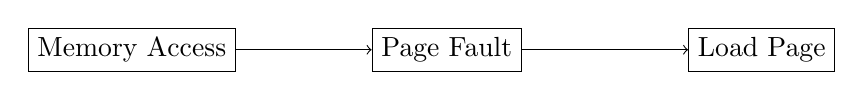
\begin{tikzpicture}
\node[draw] (cpu) at (0,0) {Memory Access};
\node[draw] (fault) at (4,0) {Page Fault};
\node[draw] (disk) at (8,0) {Load Page};

\draw[->] (cpu)--(fault);
\draw[->] (fault)--(disk);
\end{tikzpicture}
\caption{Page Fault Generation}
\end{figure}

\section{Page Fault Handling Procedure}

When a page fault occurs:

\begin{enumerate}
\item CPU generates trap
\item Kernel gains control
\item Validate memory reference
\item Locate page on disk
\item Find free frame
\item Read page into RAM
\item Update page table
\item Restart instruction
\end{enumerate}

\subsection{Detailed Walkthrough}

Suppose:

\begin{itemize}
\item Process accesses Page 25
\item Page not present
\item Valid bit = 0
\end{itemize}

Sequence:

\begin{enumerate}
\item MMU detects missing page
\item Trap generated
\item OS checks legality
\item Page located in swap area
\item Free frame allocated
\item Disk I/O performed
\item Page table updated
\item Process resumes
\end{enumerate}

\begin{figure}[H]
\centering
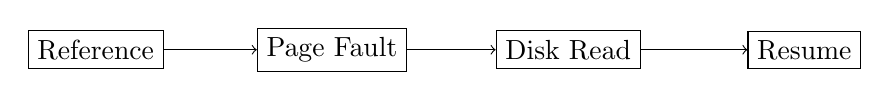
\begin{tikzpicture}
\node[draw] (a) at (0,0) {Reference};
\node[draw] (b) at (3,0) {Page Fault};
\node[draw] (c) at (6,0) {Disk Read};
\node[draw] (d) at (9,0) {Resume};

\draw[->] (a)--(b);
\draw[->] (b)--(c);
\draw[->] (c)--(d);
\end{tikzpicture}
\caption{Page Fault Handling Sequence}
\end{figure}

\section{Valid and Invalid References}

\subsection{Valid Reference}

Reference belongs to process address space.

Example:

\[
0x00400000
\]

inside allocated memory.

\subsection{Invalid Reference}

Reference outside process address space.

Example:

\[
0xFFFFFFFFFFFFFFFF
\]

Results:

\begin{itemize}
\item Segmentation fault
\item Access violation
\item Process termination
\end{itemize}

\section{Copy-on-Write (COW)}

Copy-on-Write delays copying until modification occurs.

\subsection{Motivation}

Traditional fork:

\begin{itemize}
\item Copy entire address space
\item Expensive operation
\end{itemize}

COW:

\begin{itemize}
\item Share pages initially
\item Copy only on write
\end{itemize}

\subsection{Operation}

Parent and child share page:

\begin{figure}[H]
\centering
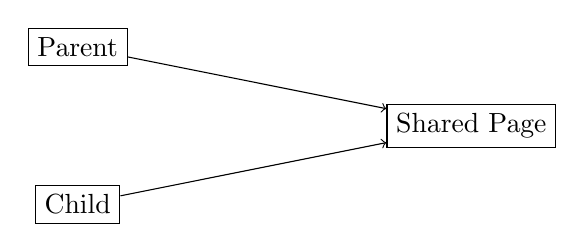
\begin{tikzpicture}
\node[draw] (p) at (0,1) {Parent};
\node[draw] (c) at (0,-1) {Child};
\node[draw] (page) at (5,0) {Shared Page};

\draw[->] (p)--(page);
\draw[->] (c)--(page);
\end{tikzpicture}
\caption{Copy-on-Write Shared Page}
\end{figure}

When child writes:

\begin{enumerate}
\item Page fault occurs
\item New page allocated
\item Data copied
\item Child receives private copy
\end{enumerate}

\section{Memory Mapped Files}

Files can be mapped directly into virtual memory.

Advantages:

\begin{itemize}
\item Faster I/O
\item Shared access
\item Simpler programming
\end{itemize}

\subsection{Example}

\begin{lstlisting}[style=interviewcode,language=C++]
int fd = open("data.txt", O_RDONLY);

void* ptr = mmap(
    NULL,
    size,
    PROT_READ,
    MAP_SHARED,
    fd,
    0
);
\end{lstlisting}

\section{Shared Memory}

Shared memory enables multiple processes to access common memory regions.

Benefits:

\begin{itemize}
\item Fast IPC
\item Low overhead
\item High throughput
\end{itemize}

\begin{figure}[H]
\centering
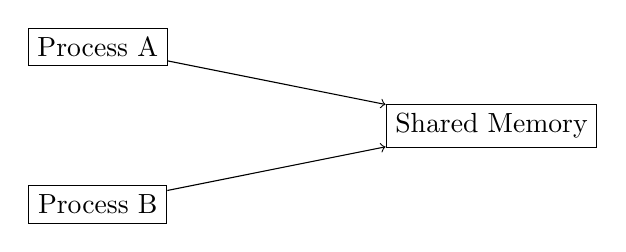
\begin{tikzpicture}
\node[draw] (p1) at (0,1) {Process A};
\node[draw] (p2) at (0,-1) {Process B};
\node[draw] (mem) at (5,0) {Shared Memory};

\draw[->] (p1)--(mem);
\draw[->] (p2)--(mem);
\end{tikzpicture}
\caption{Shared Memory}
\end{figure}

\section{Working Set Model}

Working Set = Pages actively used by a process during a time interval.

Notation:

\[
WSS_i
\]

where:

\[
WSS = Working\ Set\ Size
\]

Benefits:

\begin{itemize}
\item Prevents thrashing
\item Improves performance
\item Better memory allocation
\end{itemize}

\section{Thrashing}

Thrashing occurs when excessive page faults consume most CPU time.

Symptoms:

\begin{itemize}
\item High disk activity
\item Low CPU utilization
\item Poor throughput
\end{itemize}

\begin{figure}[H]
\centering
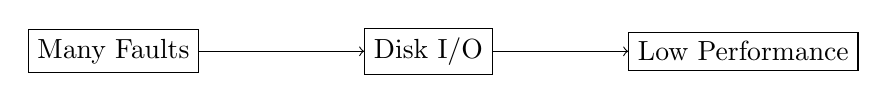
\begin{tikzpicture}
\node[draw] (faults) at (0,0) {Many Faults};
\node[draw] (io) at (4,0) {Disk I/O};
\node[draw] (slow) at (8,0) {Low Performance};

\draw[->] (faults)--(io);
\draw[->] (io)--(slow);
\end{tikzpicture}
\caption{Thrashing Cycle}
\end{figure}

\subsection{Solutions}

\begin{itemize}
\item Increase memory
\item Working set model
\item Better allocation policies
\item Reduce multiprogramming level
\end{itemize}

\section{Local Allocation Policies}

Processes receive a fixed set of frames.

Advantages:

\begin{itemize}
\item Isolation
\item Predictability
\end{itemize}

Disadvantages:

\begin{itemize}
\item Possible underutilization
\end{itemize}

\section{Global Allocation Policies}

Frames may be taken from any process.

Advantages:

\begin{itemize}
\item Better utilization
\item Adaptive allocation
\end{itemize}

Disadvantages:

\begin{itemize}
\item Unpredictable behavior
\end{itemize}

\begin{center}
\begin{tabular}{lll}
\toprule
Policy & Advantage & Disadvantage\\
\midrule
Local & Isolation & Less Flexible\\
Global & Better Utilization & Interference\\
\bottomrule
\end{tabular}
\end{center}

\section{Overcommitment}

Operating systems may allocate more virtual memory than available physical memory.

Example:

\[
64GB\ Virtual
\]

with:

\[
16GB\ RAM
\]

Advantages:

\begin{itemize}
\item Efficient resource usage
\item Supports large workloads
\end{itemize}

Risks:

\begin{itemize}
\item Thrashing
\item OOM situations
\end{itemize}

\section{Swap Space}

Swap space stores inactive pages on disk.

\subsection{Purpose}

\begin{itemize}
\item Extend apparent memory
\item Support demand paging
\item Handle memory pressure
\end{itemize}

\subsection{Drawbacks}

\begin{itemize}
\item Disk is slower than RAM
\item Excessive swapping hurts performance
\end{itemize}

\section{Virtual Memory in Linux}

Linux uses:

\begin{itemize}
\item Demand paging
\item Copy-on-write
\item mmap()
\item Shared memory
\item Swap partitions/files
\item Transparent Huge Pages
\end{itemize}

\subsection{Linux Commands}

Check memory:

\begin{lstlisting}[style=interviewcode,language=bash]
free -h
\end{lstlisting}

View mappings:

\begin{lstlisting}[style=interviewcode,language=bash]
cat /proc/self/maps
\end{lstlisting}

Check virtual memory:

\begin{lstlisting}[style=interviewcode,language=bash]
vmstat
\end{lstlisting}

\section{Virtual Memory in Windows}

Windows uses:

\begin{itemize}
\item Demand paging
\item Pagefile.sys
\item Working sets
\item Memory-mapped files
\item Copy-on-write
\end{itemize}

\subsection{Important Components}

\begin{itemize}
\item Virtual Memory Manager
\item Pagefile
\item Working Set Manager
\item Memory Compression
\end{itemize}

\section{Case Study: Launching a Large Application}

Suppose a browser executable is 500 MB.

Without virtual memory:

\begin{itemize}
\item Entire executable loaded
\item Slow startup
\end{itemize}

With virtual memory:

\begin{itemize}
\item Only necessary pages loaded
\item Remaining pages fetched on demand
\item Faster startup
\end{itemize}

\section{Case Study: fork() in Linux}

Without COW:

\begin{itemize}
\item Entire process copied
\item High overhead
\end{itemize}

With COW:

\begin{itemize}
\item Shared pages
\item Copy only when modified
\item Significant performance gain
\end{itemize}

\section{Interview Focus: What Happens During a Page Fault?}

Expected answer:

\begin{enumerate}
\item Memory reference occurs
\item MMU checks page table
\item Page absent
\item Trap generated
\item OS validates reference
\item Page fetched from disk
\item Page table updated
\item Instruction restarted
\end{enumerate}

\section{Interview Focus: Why Virtual Memory Exists}

Key points:

\begin{itemize}
\item Larger logical memory
\item Process isolation
\item Efficient memory usage
\item Multiprogramming support
\item Demand loading
\end{itemize}

\section{Interview Focus: How Copy-on-Write Works}

Key points:

\begin{enumerate}
\item Parent forks child
\item Pages shared as read-only
\item Write attempt causes fault
\item OS allocates new page
\item Data copied
\item Writer gets private page
\end{enumerate}

\section{Key Takeaways}

\begin{keytakeaways}
Virtual memory provides the illusion of a large, private address space for each process. Demand paging loads pages only when needed. Page faults occur when referenced pages are absent from memory. Copy-on-write dramatically reduces process creation overhead. Working set models help prevent thrashing. Linux and Windows both rely heavily on virtual memory mechanisms including paging, swapping, memory-mapped files, and shared memory.
\end{keytakeaways}

\section{Interview Questions with Answers}

\begin{enumerate}
\item What is virtual memory?\\
An abstraction that provides large logical memory using RAM and secondary storage.

\item Why is virtual memory needed?\\
To support large programs and efficient memory utilization.

\item What is demand paging?\\
Loading pages only when referenced.

\item What is demand segmentation?\\
Loading segments only when required.

\item What is lazy loading?\\
Deferring loading until first use.

\item What is a page fault?\\
A reference to a page not currently in memory.

\item What causes page faults?\\
Demand paging, swapping, COW, invalid references.

\item What is copy-on-write?\\
Delayed copying until modification.

\item Why is COW useful?\\
Reduces memory and fork overhead.

\item What is shared memory?\\
Memory accessible by multiple processes.

\item What is mmap?\\
Memory-mapped file mechanism.

\item What is swap space?\\
Disk space used for inactive pages.

\item What is thrashing?\\
Excessive paging causing poor performance.

\item Symptoms of thrashing?\\
High page faults and low CPU utilization.

\item What is a working set?\\
Pages actively used by a process.

\item What is overcommitment?\\
Allocating more virtual memory than physical memory.

\item What is local allocation?\\
Fixed frames per process.

\item What is global allocation?\\
Frames shared among processes.

\item What happens after a page fault?\\
OS loads page and resumes execution.

\item What is a valid reference?\\
Reference inside process address space.

\item What is an invalid reference?\\
Reference outside legal address space.

\item What is Pagefile.sys?\\
Windows swap storage.

\item How does Linux support virtual memory?\\
Demand paging, swap, mmap, COW.

\item How does Windows support virtual memory?\\
Working sets, pagefile, demand paging.

\item Most important VM interview topic?\\
Page fault handling.
\end{enumerate}

\section{MCQs with Answers}

\begin{enumerate}
\item Virtual memory primarily provides:
\begin{enumerate}[label=(\alph*)]
\item Larger Logical Memory
\item Faster CPU
\item Larger Cache
\item More Registers
\end{enumerate}
Answer: (a)

\item Demand paging loads pages:
\begin{enumerate}[label=(\alph*)]
\item At Boot
\item During Compilation
\item On Demand
\item Never
\end{enumerate}
Answer: (c)

\item A page fault occurs when:
\begin{enumerate}[label=(\alph*)]
\item Page Missing
\item CPU Fails
\item Cache Miss
\item Thread Blocks
\end{enumerate}
Answer: (a)

\item Copy-on-write delays:
\begin{enumerate}[label=(\alph*)]
\item Execution
\item Scheduling
\item Copying
\item Compilation
\end{enumerate}
Answer: (c)

\item Shared memory is used for:
\begin{enumerate}[label=(\alph*)]
\item IPC
\item Scheduling
\item Paging
\item DMA
\end{enumerate}
Answer: (a)

\item Thrashing results in:
\begin{enumerate}[label=(\alph*)]
\item Better Performance
\item More Throughput
\item Excessive Paging
\item Faster CPU
\end{enumerate}
Answer: (c)

\item Working set refers to:
\begin{enumerate}[label=(\alph*)]
\item Active Pages
\item CPU Set
\item Thread Set
\item Cache Set
\end{enumerate}
Answer: (a)

\item Swap space is located on:
\begin{enumerate}[label=(\alph*)]
\item RAM
\item Disk
\item Cache
\item CPU
\end{enumerate}
Answer: (b)

\item mmap is used for:
\begin{enumerate}[label=(\alph*)]
\item Memory Mapping
\item Scheduling
\item DMA
\item Networking
\end{enumerate}
Answer: (a)

\item Linux supports:
\begin{enumerate}[label=(\alph*)]
\item COW
\item mmap
\item Demand Paging
\item All
\end{enumerate}
Answer: (d)

\item Windows uses:
\begin{enumerate}[label=(\alph*)]
\item Pagefile
\item Working Sets
\item Demand Paging
\item All
\end{enumerate}
Answer: (d)

\item Invalid references typically cause:
\begin{enumerate}[label=(\alph*)]
\item Segmentation Fault
\item Reboot
\item Deadlock
\item Paging
\end{enumerate}
Answer: (a)

\item COW is heavily used during:
\begin{enumerate}[label=(\alph*)]
\item fork()
\item exec()
\item boot()
\item compile()
\end{enumerate}
Answer: (a)

\item Overcommitment may cause:
\begin{enumerate}[label=(\alph*)]
\item Thrashing
\item Deadlock
\item Starvation
\item DMA
\end{enumerate}
Answer: (a)

\item Demand paging improves:
\begin{enumerate}[label=(\alph*)]
\item Startup Time
\item CPU Frequency
\item Cache Size
\item Registers
\end{enumerate}
Answer: (a)

\item Working set helps prevent:
\begin{enumerate}[label=(\alph*)]
\item Thrashing
\item Scheduling
\item Deadlock
\item DMA
\end{enumerate}
Answer: (a)

\item Global allocation:
\begin{enumerate}[label=(\alph*)]
\item Shares Frames
\item Fixed Frames
\item No Frames
\item Dedicated CPU
\end{enumerate}
Answer: (a)

\item Local allocation:
\begin{enumerate}[label=(\alph*)]
\item Fixed Frames
\item Shared Frames
\item Shared CPU
\item Shared Cache
\end{enumerate}
Answer: (a)

\item Page fault generates:
\begin{enumerate}[label=(\alph*)]
\item Trap
\item Thread
\item DMA
\item Cache Line
\end{enumerate}
Answer: (a)

\item Shared memory offers:
\begin{enumerate}[label=(\alph*)]
\item Fast IPC
\item Slow IPC
\item No IPC
\item CPU Scheduling
\end{enumerate}
Answer: (a)

\item Virtual memory improves:
\begin{enumerate}[label=(\alph*)]
\item Multiprogramming
\item Isolation
\item Utilization
\item All
\end{enumerate}
Answer: (d)

\item Demand segmentation loads:
\begin{enumerate}[label=(\alph*)]
\item Segments on Demand
\item Entire Program
\item Entire RAM
\item Entire Disk
\end{enumerate}
Answer: (a)

\item Thrashing causes:
\begin{enumerate}[label=(\alph*)]
\item Low CPU Utilization
\item High CPU Utilization
\item Faster Execution
\item No Faults
\end{enumerate}
Answer: (a)

\item Pagefile.sys belongs to:
\begin{enumerate}[label=(\alph*)]
\item Linux
\item Windows
\item Android
\item BIOS
\end{enumerate}
Answer: (b)

\item Most important VM event:
\begin{enumerate}[label=(\alph*)]
\item Page Fault
\item DMA
\item Scheduling
\item Compilation
\end{enumerate}
Answer: (a)
\end{enumerate}

\section{Revision Notes}

\begin{revisionnotes}
\item Virtual memory provides larger logical address spaces.
\item Demand paging loads pages only when needed.
\item Lazy loading delays resource loading.
\item Page faults trigger OS intervention.
\item Valid references belong to allocated memory.
\item Invalid references cause faults.
\item Copy-on-write reduces fork overhead.
\item Shared memory enables fast IPC.
\item Memory mapped files simplify file access.
\item Working set represents active pages.
\item Thrashing results from excessive paging.
\item Local allocation uses fixed frames.
\item Global allocation shares frames dynamically.
\item Swap space extends apparent memory.
\item Linux and Windows both rely heavily on virtual memory.
\end{revisionnotes}

\section{Cheat Sheet}

\begin{longtable}{|p{5cm}|p{8cm}|}
\hline
Concept & Summary \\
\hline
Virtual Memory & Large logical memory abstraction \\
\hline
Demand Paging & Load pages when needed \\
\hline
Demand Segmentation & Load segments on demand \\
\hline
Lazy Loading & Deferred loading \\
\hline
Page Fault & Missing page reference \\
\hline
COW & Copy only upon modification \\
\hline
mmap & Memory mapped files \\
\hline
Shared Memory & Fast IPC mechanism \\
\hline
Working Set & Active page collection \\
\hline
Thrashing & Excessive paging activity \\
\hline
Local Allocation & Fixed frames per process \\
\hline
Global Allocation & Shared frame pool \\
\hline
Swap Space & Disk-backed memory extension \\
\hline
Linux VM & Demand paging + COW + mmap \\
\hline
Windows VM & Pagefile + working sets \\
\hline
Page Fault Flow & Trap $\rightarrow$ Load $\rightarrow$ Resume \\
\hline
Main Interview Topic & Page Fault Handling \\
\hline
COW Benefit & Reduced fork cost \\
\hline
Thrashing Fix & Working set control \\
\hline
VM Goal & Efficient memory utilization \\
\hline
\end{longtable}